% Source : http://forum.mathematex.net/latex-f6/tableaux-de-proportionnalite-t3752.html?hilit=tableau

\documentclass[]{article}
	\usepackage{tikz,pgflibraryshapes}


\begin{document}

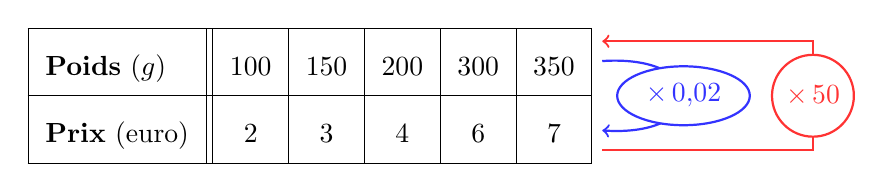
\begin{tikzpicture}
% Création du tableau dans un nœud
	\node[anchor=east,rectangle,inner sep=0pt,outer sep=0pt]%
	(Tbl) {%
		\renewcommand{\arraystretch}{2}%
		\begin{tabular}{|l||c|c|c|c|c|}%
			\hline%
			\textbf{Poids} $(g)$&100 & 150 & 200 & 300 & 350 \\%
			\hline%
			\textbf{Prix} (euro)& 2 & 3 & 4 & 6 & 7 \\%
			\hline%
		\end{tabular}%
	};

% Positionnement des points d'ancrage des flèches
	\path (Tbl.north east) -- (Tbl.south east) %
	node[pos=0.10](Fl_R){}% départ flèche rectangulaire
	node[pos=0.25](Fl_C){}% départ flèche courbe
	node[pos=0.75](C_lF){}% pointe flèche rectangulaire
	node[pos=0.9](R_lF){};% pointe  flèche courbe

% Flèche courbe
	\draw[->,line width=.8pt,blue!80](Fl_C) .. controls +(1.5cm,.1cm) and +(1.5cm,-.1cm)..
	node[ellipse,fill=white,draw]{$\times\,0{,}02$} (C_lF);

% Flèche rectangulaire
	\draw[<-,line width=.8pt,red!80](Fl_R) -| (2.8cm,0cm)
	node[circle,fill=white,draw]{$\times\,50$}|-(R_lF) ;
\end{tikzpicture}

\end{document}